\chapter{Inledning}

En drönare är ett obemannat luftfordon som kan styras med hjälp av visionsbaserad-, tröghets- eller satellitnavigation \citep{geospatial}. För att en drönare skulle kunna navigera autonomiskt måste den vara medveten om sitt läge, omgivning, hastighet, kursriktning samt start- och slutplats. Andra faktorer som borde beaktas för att flyga från start till slutplatsen är hur drönare kan behandla data från inbyggda sensorer i sig, det vill säga kartlägga miljön och sin egen position i denna miljö samt hur man planerar vägen utan att kollidera med hinder.

För att drönare är mer versatila än robotar som inte flyger så finns det särskilda användningsfall för dem. De kan övervaka markföroreningar, industriolyckor eller växternas behov av vatten och näring \citep{crowdsurveillance}. Drönare har också använts vid katastrofområden, såsom vid jordbävningen nära Japan för att mäta strålningsvärden nära Fukushima och att få visuell information om katastrofområdet samt i räddning av invandrare vid medelhavet. Inom logistikbranschen är man intresserad om autonoma drönaren som skulle leverera paket för kunder, till exempel 86 \% av Amazons paket väger mindre än 5 skålpund (ca. 2.26 kg) och de har tänkt på att leverera paket inom 30 minuter för människor som bor nära Amazons lager \citep{cbsnews}. Lovande forskning för autonoma robotar är inom visionsbaserad navigering med hjälp av datorseende.

Robotnavigering med hjälp av datorseende är ett aktivt forskningsområde \citep{982903}. För att robotar skulle vara verkligen autonoma måste de kunna kartlägga sin omgivning och lokalisera sig själv i omgivningen, detta kallas för SLAM (Simultaneous Localization and Mapping). SLAM är ett problem som har fått uppmärksamhet av det vetenskapliga samfundet sedan 80-talet och har sätts som ett rön om det löses. Utmaningar i utvecklingen är att konstruera algoritmer som fungerar i allmänhet, såsom i dynamiska och stora miljön \citep{realslamproblem}. Sannolikhetsberäkning är tillvägagångssättet för att lösa SLAM-problemet och flesta av de algoritmer som har löst problemet baserar sig på sannolikhetsberäkning \citep{ProbabilisticRobotics}.

Avhandlingen kommer att vara en översikt om SLAM problemet och vilka metoder det finns för att kartlägga miljön och lokalisera sig själv med hjälp av datorseende. Frågor som behandlas är: Vad är det fundamentala problemet med SLAM? Vilka SLAM metoder skulle kunna användas eller har använts med drönare och vad begränsar användningen av dessa? Varför har visionsbaserad navigation fått så mycket uppmärksamhet än de traditionella metoderna?

Resten av avhandlingen är strukturerad enligt följande: I kapitel 2 öppnas bakgrund bakom visionsbaserad navigering. Vad är visionsbaserad navigering och vilka sensorer kan användas samt vilka metoder det finns för att extrahera data ur bilder. Kapitel 2 kommer också att innehålla basen för de flesta lokaliseringsalgoritmer som baserar sig på sannolikhetsberäkning och vad vi menar med kartläggning. Dessa är nödvändiga att förstå SLAM problemet. Kapitel 3 är om samtidig lokalisering och kartläggning och hur SLAM problemet kan grupperas i olika kategorier enligt data som man har. Kapitel 3 kommer också att innehålla användningsfall för några av de metoderna. Kapitel 4 är en sammanfattning om avhandlingen.

\chapter{Bakgrund}

\section{Navigering}

Med navigering anser vi att en drönare planerar och utför en rutt från startplats till målet \citep{geospatial}. För att kunna navigera till målet måste den vara medveten om sitt läge, miljö, kursriktning och hastighet. Autonom navigering för drönare kräver att den kan undvika hinder, planera sin rutt samt ta omvägar vid behov. I visionsbaserad navigering används visuella sensorer för att få bilder som indata. Bilderna kan sedan behandlas med algoritmer för att få en representation av omgivningen och lokalisera drönare i omgivningen. 

Visuella sensorer som kan användas är monokulära, stereo, RGB-D och fisheye-kameror samt kombinationer av dessa \citep{geospatial}. Kamerasensorer är billiga att operera, väger lite och med dem kan man uppfatta till exempel färg, textur och former. Med traditionella navigeringsmetoder, såsom satellitnavigering som använder GPS-signaler (Global Positioning System) för lokalisering, och tröghetsnavigering (Inerital Navigation System) som använder accelerometer och gyroskop, får man inte visuell information av omgivningen. Med kameror kan man navigera i GPS-förnekade områden för att kameror är passiva, det vill säga de kan inte bli störda av utomstående signaler eller upptäckas av utomstående entitet. Med visionsbaserad navigering som använder kameror så är en drönare inte beroende på utomstående hjälp, därmed kan man beräkna drönarens position i omgivningen inombords \citep{opticalflowuav}.

Drönare kan använda laser- och ultraljudsensorer för att navigera, men dessa kräver mer energi och väger mer än kameror \citep{6385934}. För att drönare byggs mindre än förr, och på grund av detta har begränsad bärförmåga samt batterikapacitet, har dessa sensorer uteslutnas. Med hjälp av visionsbaserad navigering som använder sig av kameror kan man få rikligt med information om omgivningen \citep{geospatial}. Visionsbaserad navigering, som är ett aktivt forskningsområde, är en av de mest lovande metod för robotnavigering.

\section{Datorseende och bildbearbetning}

Med datorseende kan man få sekventiella bilder ur omgivningen som sedan kan bearbetas med algoritmer \citep{982903}. Bildbearbetning i visionsbaserad navigering betyder att man gör utdrag ur bilder i form av former, kanter, linjer, djuphet, rörelse, färg eller mönster. Då man extraherar egenskaper ur bilder är det möjligt att utjämna bilder \citep{mapbuildingsift}. Detta menar att man gör bilder otydligare för att få bort digitalt brus och att bilden har mindre detalj. Då man extraherar egenskaper med algoritmer ur bilder som är otydligare får man färre, men bättre träffar. Metoder för att uppskatta djuphet med datorseende är att beräkna binokulära skillnaden eller rörelseparallax \citep{suomimainittu}. 

Rörelseparallax betyder att objekt rör på sig snabbare i synfältet då de är närmare observatören och långsammare då de är långt borta, detta gäller också om observatören rör på sig och objektet står stilla \citep{suomimainittu, parallax}. För att räkna binokulära skillnaden för observerade kännetecken behöver man två kameror som är riktade parallellt i samma linje så att deras synfält överlappar, kamerornas distans från varandra är känd och av båda kamerornas bilder utdras samma kännetecken. Från skillnaden ur kännetecknets horisontala position i båda av kamerornas bilder kan man estimera djuphet. Med en monokulär kamera kan man uppskatta djuphet av bilder baserat på rörelseparallax. För att estimera djuphet med monokulärkamera och rörelseparallax behöver man veta distansen till ett objekt då navigeringen börjar och som indata får man bilder och rörelseinformation av roboten. Rörelseinformationen i robotar på stagid grund kan man få från vägmätare och tröghetsmätare som är inbyggt i roboten.

\cite{suomimainittu} undersökte detta och märkte att stereokameror fungerar bättre då objekten är nära medan monokulära kameror med hjälp av rörelseparallax kan uppfatta mer precis distans då distansen växer \citep{suomimainittu}. Med stereokamera kan djupheten estimeras bra upp till cirka 10 meters avstånd och vid 20 meters avstånd så är estimeringarna oanvändbara, efter detta måste man växla över till att använda monokulära kameran. \cite{suomimainittu} skriver att i framtiden kommer de att forska hur de kan beräkna rörelseinformationen från stereokamerornas bilder så att de kan avlägsna tröghets- och vägmätaren. Detta ger möjlighet att estimera djuphet till exempel för drönare.

Fast man har fördelar på data som man kan extrahera ur kameror jämfört med andra sensorer som till exempel laser och ultraljud, så med kameror är förändring i belysning, vädret och årstid samt skuggor ett problem som måste tas i beaktande, för det mesta då man navigerar utomhus \citep{982903}. Dessa problem har lösts med att bearbeta bildernas färgnyanser, färgmättnad (saturation) och ljusstyrka.

För att få former, kanter eller linjer ur bilder finns det olika algoritmer såsom SIFT (Scale-Invariant Feature Transform), HARRIS hörn upptäckare, SURF (Speeded Up Robust Features), ORB (Oriented FAST and Rotated BRIEF), med mera \citep{orb, slamproblem, mapbuildingsift}. SIFT, SURF och ORB prövar hitta egenskaper från bilderna som är invariant för rotation, som menar att samma egenskaper kan hittas från olik synvinkel \citep{orb}. Enligt \cite{orb} är ORB mer energieffektiv algoritm än SIFT för att den kräver mindre beräkning för att extrahera egenskaper ur bilder, som betyder att den är snabbare färdig, utan att tappa effektivitet.

\section{Lokalisering i omgivningen}

Med att en robot lokaliserar sig själv menar vi att den tar reda på sin position i miljön \citep{982903}. Då man har en uppfattning om miljön, det vill säga en karta, så kan en drönare lokalisera sig själv med att ge den landmärken som den hittar då den navigerar eller så kan den observera dessa själv och associera dem med kartan som den har. Från bilderna ur kamerorna i drönaren identifieras landmärken, sedan matchas observerade landmärken med de som finns i kartan och efter det kan man estimera positionen av roboten.

Då roboten navigerar så beräknas positionen och orientationen av roboten med sannolikhetsberäkning baserat på tid och indata av sensorer \citep{ProbabilisticRobotics}. Under navigeringen vill roboten estimera sin position efter varje rörelse. Detta gör den med att estimera vart rörelseorder kommer att ta den och efter att den har rört på sig observerar den landmärken. Med att den observerar landmärken efter rörelsen kan roboten förbättrar sin förtroelse om sin position. 

För att estimera detta så kan man beteckna robotens position och riktning i miljön för varje tidpunkt $t$ med $x_t$. Variabeln $x_t$ beskriver alltså robotens tillstånd, som i drönarens fall kan vara till exempel drönarens koordinater och orientering i miljön med sex frihetsgrader. Rörelseorder betecknas som $u_t$ och landmärken extraherade från kamerasensorer med $z_t$. För att $x_t$ är en möjlighet i en kontinuerlig stokastisk variabel $X$ så kan betingade sannolikhetsfördelningen för $x_t$ skrivas som följande:
\begin{align}
    P( X = x_t | x_{0:t-1}, z_{1:t-1}, u_{1:t})
\end{align}

Där vi antar att roboten rör på sig $u_1$ före den skaffar sensorinformation $z_1$. Med Markovegenskapen för $x_t$, som betyder att en villkorlig sannolikhetsfördelning för $x_t$ är bara beroende på den tidigare sannolikhet $x_{t-1}$ och inte på händelseförloppet som hände före $x_{t-1}$. Då $x_t$ är den bästa framtidssyn så kan vi begränsa att $x_t$ är beroende bara på den tidigare position $x_{t-1}$ och rörelseinformation $u_t$, se figur \ref{markov}. Betingade sannolikhetsfördelningen för $x_t$ kan då betecknas som följande:
\begin{align}
    P(x_t | x_{t-1} u_{t})
\end{align}

Då $x_t$ har Markovegenskapen så är betingade sannolikhetsfördelningen för observerade landmärken $z_t$:
\begin{align}
    P(z_t | x_{0:t}, z_{1:t-1}, u_{1:t}) = P(z_t|x_t)
\end{align}

\begin{figure}[ht]
    %\begin{figure}[tbh] t= top, b = bottom, h=here
    \begin{center}
    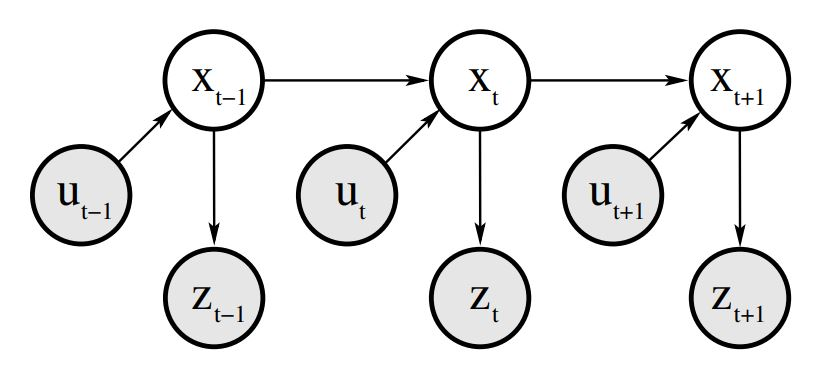
\includegraphics[width=0.75\textwidth]{markov.JPG}
    \caption{En graf om lokalisering som visualiserar Markovegenskapen där till exempel $x_t$ är bara beroende av $x_{t-1}$ och $u_t$, detta kallas också för en Markovkedja \citep{ProbabilisticRobotics}.}
    \label{markov}
    \end{center}
\end{figure}

$P(x_t|x_{t-1}, u_{t})$ är rörelseuppfattningssannolikhet och $P(z_t|x_t)$ är landmärkesuppfattningssannolikhet för roboten \citep{ProbabilisticRobotics}. 

Positionen och riktning av roboten kan beräknas med Bayes filter som använder sig av rörelse- och landmärkesuppfattningssannolikhet \citep{ProbabilisticRobotics}. Bayes filter är en rekursiv algoritm som beräknar aposteriorisannolikhet för robotens position $bel(x_t)$ baserat på robotens tidigare position $bel(x_{t-1})$, rörelseinformation $u_t$ och observerade landmärken $z_t$. Med hjälp av Bayes regler, lagen om total sannolikhet för kontinuerliga variabler och Markovegenskapen kan detta bevisas med matematisk induktion där vi antar att $x_t$ har Markovegenskapen och att $bel(x_0)$ sannolikhetsfunktion är känd då $t = 0$. Med att sannolikhetsfunktionen är känd menar vi att roboten vet sin position vid början med full säkerhet eller så är $bel(x_0)$ en likformig sannolikhetsfördelning.
\begin{align}
bel(x_t) & = P(x_t | z_{1:t}, u_{1:t}) \tag{BF1}\label{BF1} \\
        & = \eta P(z_t | x_t, z_{1:t-1}, u_{1:t}) P(x_t | z_{1:t-1}, u_{1:t}) \tag{BF2}\label{BF2}\\
        & = \eta \underline{P(z_t | x_t)} P(x_t | z_{1:t-1}, u_{1:t}) \tag{BF3}\label{BF3}\\
        & = \eta P(z_t | x_t) \underline{\int P(x_t | x_{t-1}, z_{1:t-1}, u_{1:t}) P(x_{t-1} | z_{1:t-1}, u_{1:t}) dx_{t-1}} \tag{BF4}\label{BF4}\\
        & = \eta P(z_t | x_t) \int \underline{P(x_t | x_{t-1}, u_t)} P(x_{t-1} | z_{1:t-1}, u_{1:t}) dx_{t-1} \tag{BF5}\label{BF5}\\
        & = \eta P(z_t | x_t) \int P(x_t | x_{t-1}, u_t) P(x_{t-1} | z_{1:t-1}, \underline{u_{1:t-1}}) dx_{t-1} \tag{BF6}\label{BF6}\\
        & = \eta P(z_t | x_t) \int P(x_t | x_{t-1}, u_t) \underline{bel(x_{t-1})} dx_{t-1} \tag{BF7}\label{BF7}
\end{align}

Bayes filters definition är \ref{BF1}, det vill säga förtroende för roboten att den är vid $x_t$, som betecknas $bel(x_t)$, är samma som sannolikheten av $x_t$ givet $z_{1:t}$ och $u_{1:t}$. Med Bayes teorem kan detta skrivas om i format \ref{BF2}. Vid \ref{BF3} använder vi Markovegenskapen för $x_t$ så kan betingade sannolikheten för $z_t$ skrivas som landmärkesuppfattningssannolikheten. Med satsen om total sannolikhet för kontinuerliga variabler, som uttrycker sannolikhet för enskilda händelser till betingade sannolikhet, kan formeln skrivas om till \ref{BF4}. Vid \ref{BF5} och \ref{BF6} använder vi Markovegenskapen för $x_t$, se Markovkedjan i figur \ref{markov}. Till slut får vi \ref{BF7}, som bevisar med induktion att algoritmen fungerar rekursivt \citep{ProbabilisticRobotics}.

Bayes filters algoritmen fungerar så att för varje $x_t$ beräknas två kritiska steg, som är spådom och korrigering \citep{ProbabilisticRobotics}. Spådomsdelen i algoritmen är delen där vi beräknar integralen för två faktorer: sannolikheten att rörelseinformationen $u_t$ tar oss till $x_t$ och den gamla förtroende av positionen $bel(x_{t-1})$. Korrigeringsdelen är då man multiplicerar spådomsdelen med sannolikhet att $z_t$ skulle observeras för varje möjliga $x_t$. Oftast är korrigeringsdelen inte en sannolikhet, alltså täthetsfunktionens summa är inte 1 för varje värde, därför används det en normering konstant $\eta$ för att normera sannolikheten. Ett steg av algoritmen är definierat nedan, se algoritmen \ref{BFA}, som sedan görs rekursivt för resultatet av algoritmen och när man har ny rörelseinformation och landmärken. Utmaning i algoritmen är integralen i spådomsdelen. Man borde begränsa robotens tillstånd att vara en ändlig variabel så att integralen över spådomsdelen blir en summa. 

\begin{algorithm}[H]
    \SetAlgoLined
    \SetAlgoRefName{BFA}
    \label{BFA}
    \FuncSty{BayesFilter($bel(x_{t-1})$, $u_t$, $z_t$):} \\
    \ForAll{$x_t$}{
        $spådom$ = $\int P(x_t | x_{t-1}, u_t) bel(x_{t-1}) dx_{t-1}$ \\
        $bel(x_t)$ = $\eta P(z_t | x_t)$ $spådom$
    }
    \Return{$bel(x_t)$}
    \caption{Bayes Filter Algoritm}
\end{algorithm}

Bayes filter är huvudsakliga algoritmen för att beräkna robotens position och riktning \citep{ProbabilisticRobotics}. Algoritmen baserar sig starkt på Markovegenskapen att det nuvarande läge är oberoende av tidigare data. I robotnavigering är det inte dock så lätt att anta detta, för det skulle betyda att allt runtomkring roboten borde vara statiskt. Till exempel om en bil rör på sig då roboten navigerar så då man gör landmärkesuppfattning kommer Bayes filter att ge felaktig estimering. Bayes filtern är också basis för många andra lokaliseringsalgoritmer, som till exempel Kalman filter eller Markov lokalisation. Oftast är det inte möjligt att begränsa robotens tillstånd så att integralen i Bayes filtern blir en summa över spådomsdelen. Algoritmer som används för lokalisering måste därför beräkna ett approximativt värde för detta och det är här som olika lokaliseringsalgoritmer skiljer sig.

Med att approximera värdet i lokaliseringsalgoritmer så avstår man oftast från någon egenskap som är viktigt för robotnavigering, såsom beräkningseffektivitet, noggrannhet i approximeringen av tillståndet eller enkel implementering av algoritmen för robotar \citep{ProbabilisticRobotics}. 

Positionen av roboten kan beräknas också med att räkna distansen till landmärken och distansen mellan landmärken som extraheras ur bilder, alltså uppehålla en korrelationsmatris om landmärken och deras förhållande från robotens position \citep{realslamproblem, ProbabilisticRobotics}. Då man observerat stora mängder av landmärken så kommer beräkningsbehovet att växa kvadratiskt enligt observerade landmärken. 

Lokalisering kan delas i global och lokal lokalisering \citep{982903, globalsubmaps}. Med global lokalisering har roboten ingen vetskap om sin position i början av navigeringen. I lokal lokalisering har roboten en ungefärlig eller exakt vetskap om sin plats vid början av navigeringen som den fått som indata. Lokala lokaliseringsmetoder strävar för att korrigera fel som uppstår av robotens rörelse. Globala lokaliseringsmetoder kan återvinna från verkliga misstag då man estimerar robotens position. Global och lokal lokalisering är då täthesfunktionen av den första förtroende om robotens position i miljön, som till exempel i Bayes filtern vore $bel(x_0)$ \citep{ProbabilisticRobotics}.

\section{Kartläggning av omgivningen}

Med kartläggning av omgivningen anser vi att roboten kartlägger sin omgivning med hjälp av data som den har tillgång till \citep{ProbabilisticRobotics}. Detta kan vara till exempel rörelseinformation eller sensorinformation samt kombinationer av dessa. Kartläggning är ett problem som är beroende av lokalisering. Då man har en uppfattning av robotens läge och åtkomst till rörelseinformation är kartläggning lättare än då robotens position i början är okänd. För att konstruera en karta så måste man ta i beaktande störningar som uppstår av rörelse- och sensorinformation.

En karta om miljön kan representeras i två (2D) eller tre (3D) dimensioner \citep{geospatial}. Kartor kan sparas i olika format, såsom datorstödd konstruktion (CAD, Computer-Aided Design), beläggningskarta (Occupancy Grid Map), topologisk karta eller en enkel graf om landmärken och deras sammankopplingar \citep{982903}. En datorstödd konstruktion av miljön kan vara en mycket detaljerad representation av omgivningen. En beläggningskarta är en 2D eller 3D-modell av omgivningen som är sparat i ett rutsystem där rutor som är upptagna är någon objekt i miljön \citep{6095058, 982903}. Att konstruera en 3D representation av omgivningen kräver mer beräkningskapacitet än 2D kartor, för att man tar i beaktande fler dimensioner \citep{ProbabilisticRobotics}. För robotar som navigerar på stadig grund är oftast en 2D-representation tillräckligt, men för drönaren behöver man kartlägga i 3D.

Kartan kan vara färdigt sparad för en drönare eller så kan miljön kartläggas från bilderna av sensorerna då den flyger \citep{geospatial}. Med 3D volymetriska sensorer kan man konstruera en 3D modell och spara denna information i en Octree-struktur. Med strukturen kan data om miljön packas i mindre format utan att tappa möjligheten att uppdatera informationen vid behov. En annan metod som tas upp är med stereovisionsalgoritmer göra en djuphetskarta och behandla data till plana ytor som minskar på missvisning som uppstår med användning av stereovision algoritmer när man bygger upp djuphetskartan. Viktigt i kartläggning är att kartan kan lätt uppdateras då man gör nya observationer \citep{globalsubmaps}.

Oftast så har robotar inte en färdig karta som de kan använda för att navigera och för att åstadkomma autonoma robotar så måste de kunna själv kartlägga sin omgivning \citep{ProbabilisticRobotics}. Kartläggning för robotar är ett problem som är svårt utan lokalisering, därför refereras kartläggning för robotar som samtidig lokalisering och kartläggning. 

\chapter{Samtidig lokalisering och kartläggning}

Samtidig lokalisering och kartläggning (SLAM) är ett av de grundläggande problem i robotnavigering \citep{realslamproblem}. SLAM är ett problem där en autonom robot som inte har tidigare information om sin plats eller omgivning skall samtidigt bygga en karta och lokaliserar sig själv till exempel med hjälp av att identifiera landmärken. Detta kan estimeras med sannolikhetsberäkning baserat på tid $t$, där man tar i beaktande riktningen och positionen av roboten $x_t$, distansen roboten rör på sig $u_t$, kartan $m$ och observationer för varje landmärke som roboten gör $z_t$, se figur \ref{slam-problemet}. Att beräkna robotens läge med sannolikhetsberäkning så är formeln $P(x_t, m|z_{1:t}, u_{1:t})$. 

SLAM problemet kan delas i två delar som är Fullständig SLAM och Online SLAM \citep{ProbabilisticRobotics}. Skillnaden med dessa är hur man beräknar betingade aposteriorsannolikheten för $x_t$. I fullständig SLAM beräknas betingade sannolikheten från hela robotens positionskedja $x_{1:t}$, det vill säga $P(x_{1:t}, m | z_{1:t}, u_{1:t})$, medan i online SLAM använder man bara senaste läge $x_{t-1}$, alltså Markovegenskapen. Några lösningar för SLAM som baserar sig på sannolikhetsberäkning är Extended Kalman Filter (EKF-SLAM), som är en Online SLAM-lösning, och FastSLAM, som är en fullständig SLAM-lösning \citep{realslamproblem, ProbabilisticRobotics}. 

\begin{figure}[ht]
    %\begin{figure}[tbh] t= top, b = bottom, h=here
    \begin{center}
    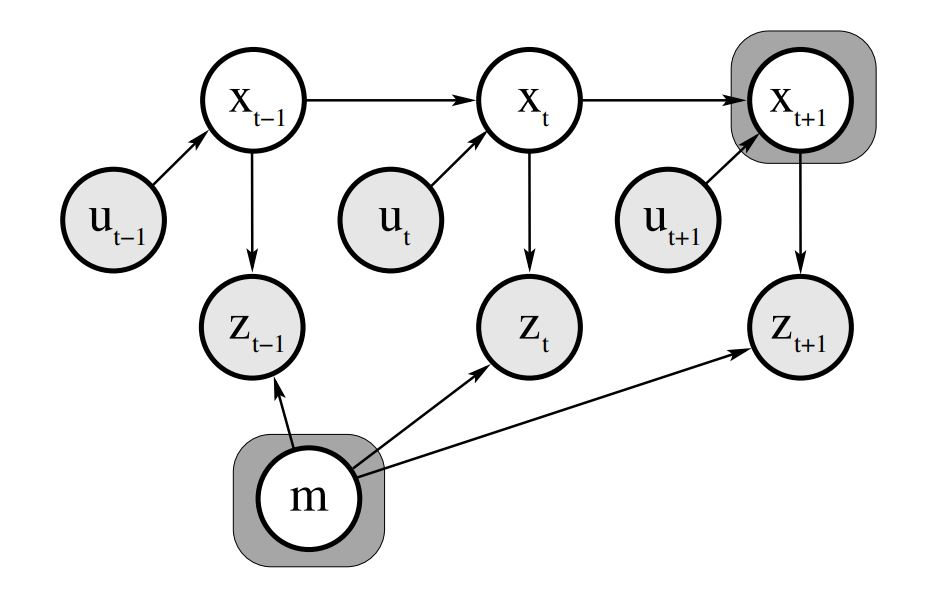
\includegraphics[width=0.8\textwidth]{online-slam.JPG}
    \caption{Bild på SLAM-problemet \citep{ProbabilisticRobotics}.}
    \label{slam-problemet}
    \end{center}
\end{figure}

SLAM-problemet har delproblem som borde lösas för att få robotar att navigera autonomiskt \citep{slamproblem}. Ett stort problem i flesta visionsbaserade SLAM-lösningar är dataföreningsproblemet, som betyder att man identifierar två olika landmärken som en och samma. Detta problem kan uppstå redan vid korta rörelsen av robotar eller då en robot har navigerat och kommer till en plats som den har redan varit i förr, detta kallas för loopstängning (Loop Closure). Med att förena landmärken fel så uppkommer det missvisningar då man estimerar positionen av roboten.

För autonom navigering behöver en robot veta sitt läge i miljön \citep{geospatial}. Med hjälp av kameror, bildbearbetning och beräkning kan miljön kartläggas, i helhet eller delvis, och drönaren lokalisera sig själv, detta kallas också för visuell lokalisering och kartläggning. Detta kan delas i tre kategorier baserat på data som man har i början av navigeringen. Kategorierna är kartlösa (mapless), kartbaserade (map-based) och kartbyggande (map-building) system. 

\section{Kartlösa system}

Kartlösa system är oftast den realistiska situationen då man navigerar och är den situationen som träffar bäst SLAM definitionen \citep{ProbabilisticRobotics}. I system utan karta navigerar drönare bara med hjälp av att observera tydliga egenskaper i miljön \citep{982903}. Dessa kan vara till exempel väggar, dörrar, möbler eller andra landmärken. Metoder som används inom kartlösa system är optiskt flöde (Optical flow) och spårning av egenskaper (Feature tracking). 

\subsection{Optiskt flöde}

Optiskt flöde hänvisar till uppfattad relativ rörelse i sekventiella bilder mellan observatören och till exempel någon fästpunkt i miljön \citep{opticalflowuav}. Rörelse uppstår i sekventiella bilder till exempel då man vänder kameran eller om något rör på sig då kameran är stilla. 

\cite{341094} har använt optiskt flöde i en robot för att imitera bin \citep{341094}. De placerade två kameror på varsin sida av en robot och beräknade hastigheten från bilderna av båda kamerorna med att ta fem bilder som utjämnas med Gaussisk oskärpa och de två sista utjämnade bilder används för att beräkna medeltalet av optiska flödesvektorer. Om flödesvektorerna var samma på båda sidorna så for roboten rakt framåt, annars så far den mot den sida vilkens hastighet är mindre. Metoden som \cite{341094} använde för roboten fungerar bara om båda kamerorna är symmetriskt riktade från varandra när man tar i beaktande rörelseriktningen av roboten. Denna teknik fungerar dåligt i strukturlösa miljö och det går inte att byta rörelseriktningen då man navigerar på detta sätt i korridorer. 

Fastän metoden som \cite{341094} använde tog bara i beaktande horisontala flödesvektorer så har sedan detta användning av optiska flödesmetoder använts i drönare \citep{6564752}. Nuförtiden kan drönare uppskatta avstånd, hålla sin höjd, undvika hinder, beräkna hastighet och landa på en plattform som rör på sig med hjälp av optiskt flöde.

\subsection{Spårning av egenskaper}

Spårning av egenskaper (Feature tracking) används för att skaffa information om objekt, så som linjer, hörn och olika former som är invariant för rörelse \citep{geospatial}. Med hjälp av dessa egenskaper av objekten och deras relativa rörelse i sekventiella bilder kan man bestämma robotens position. Då drönare navigerar i området, så kommer den troligtvis att se dessa objekt från olika perspektiv, som hjälper drönare att navigera. Traditionella SLAM-lösningar, såsom EKF-SLAM och FastSLAM faller under denna kategori \citep{voslamlatif}. Dessa SLAM-lösningar fungerar inte då det finns mycket egenskaper att extrahera i miljön. EKF-SLAM nackdel är beräkningsbehovet som växer kvadratiskt av antalet egenskaper och FastSLAM nackdel är bildbearbetning.

För att drönaren har begränsad batterikapacitet och bärkraft har \cite{voslam} föreslagit användning av VO-SLAM (Visual Odometry SLAM) som kan kartlägga omgivningen och lokalisera observatören då det finns upp till 30 000 egenskaper i kartan, med en stereokamera som tar 31 bilder per sekund och en krets som använder tio gånger färre energi än en Intel i7 3770K-processor \citep{voslam}. Deras VO-SLAM algoritm implementeras i en FPGA-krets (Field-Programmable Gate Array) vilkens logik är omprogrammerbar, den använder färre energi än vanliga processorer och kan beräkna parallellt. 

VO-SLAM-lösningen fungerar så att de extrahera landmärken med SIFT från bilderna \citep{voslam}. Med hjälp av binokulära skillnaden från bilderna i stereokameran konstruera de en 3D-representation av dessa landmärken som de sparar i en matris. FPGA-kretsen, som är byggt och programmerat för matrisberäkning, beräknar vektorvinklarna för varje observerade landmärke från globala kartan och hittar de bästa träffar för lokaliseringsalgoritmen. Före lokaliseringsuppfattningen använder de RANSAC (Random Sample Consensus) för att ta bort avvikande träffar inom landmärken, se figur \ref{voslamprocess}. 

\begin{figure}[ht]
    %\begin{figure}[tbh] t= top, b = bottom, h=here
    \begin{center}
    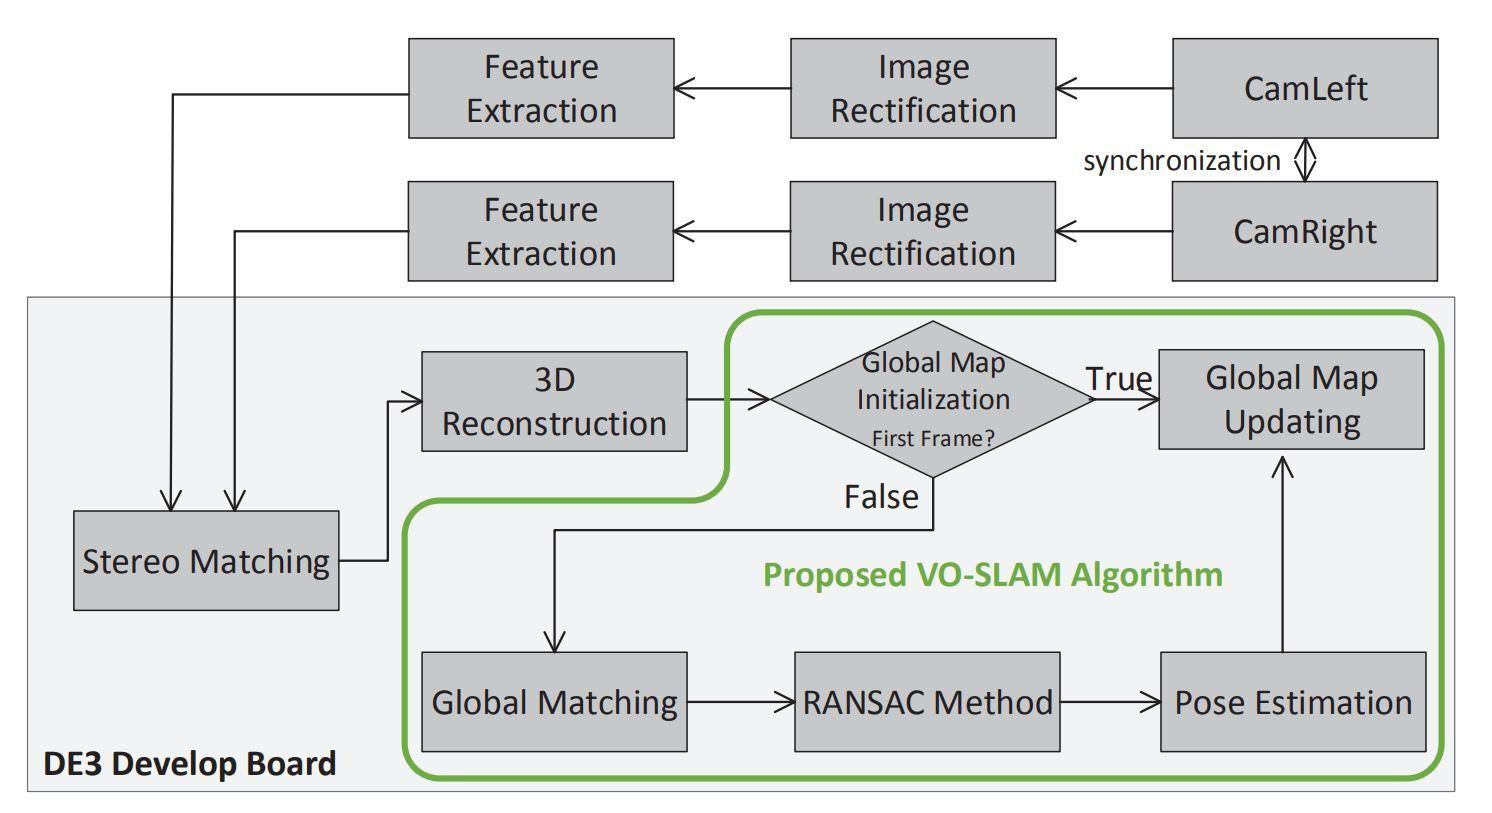
\includegraphics[width=0.75\textwidth]{voslam.JPG}
    \caption{Bild på VO-SLAM processen \citep{voslam}.}
    \label{voslamprocess}
    \end{center}
\end{figure}

Med hjälp av FPGA-kretsen har de fått dataförening med matriser att beräknas i realtid med upp till 31 bilder i sekund och litet energibehov. Enligt \cite{voslam} kan VO-SLAM estimera positionen med 1–2 cm exakthet med upp till 30 000 landmärken i kartan, hantera loopstängning och enligt dem är troligtvis en av de mest energieffektiva lösningen \citep{voslam}. Något som deras lösning tar inte i beaktande är SIFT algoritmens tidskrav. \cite{voslamlatif} använder VO-SLAM i en drönare där de delat upp processen så att indata från stereokameran, bildbearbetning och 3D-representationen, som görs med SIFT, bearbetas i en egen processor och uppdatering av kartan, matcha observerade landmärken med kartan, lokalisering och uppdatering av kartan hanteras i FPGA-kretsen \citep{voslamlatif}. 

\section{Kartbaserade system}

Med kartbaserade system har drönare en färdig vetskap om miljön som kan vara i form av geometriska modeller, topologiska kartor eller förhållande mellan landmärken \citep{982903}. Idén är att då roboten navigerar prövar den hitta till exempel landmärken från bilder som är lika till de landmärken som roboten vet om. När den förenat landmärken rätt så kan roboten estimera sin position i miljön. Med kartbaserad navigering kan en drönare planera sin rutt i förhand och beräkna omvägar under navigeringen då det behövs \citep{geospatial}. 

Kartbaserad lokalisering med datorseende kan delas upp i fyra steg, som är följande \citep{982903}:

\begin{itemize}
    \item skaffa sensorinformation av kamerorna
    \item upptäcka landmärken från informationen med bildbearbetning
    \item matcha observationerna med kartan
    \item estimera positionen av roboten
\end{itemize}

Det svåraste steget av dessa är att matcha observationerna med kartan som den har. Detta kallas för dataföreningsproblemet. Roboten kan inte med full säkerhet veta sin position och då är det svårt att matcha landmärken med kartan \citep{982903}.

Då kartan finns kan man fokusera på lokalisering av roboten \citep{982903}. I global lokalisering måste man lita på att man kan förena observationerna med informationen man har och ta i beaktande osäkerheten med att observationerna kan matcha flera av de landmärken man vet om. Globala lokaliseringsproblemet kan lösas till exempel med Monte Carlo lokalisation eller Markov lokalisation, som båda är en variant av Bayes filter som presenterades i kapitel \nameref{BFA} \citep{ProbabilisticRobotics}. 

Monte Carlo lokalisation fungerar så att en robot antar med lika sannolikhet sin position i kartan vid början av navigeringen \citep{montecarlo}. Approximerande i Monte Carlo fungerar så att roboten slumpmässigt väljer platser vart den möjligen skulle befinnas med den rörelseorder som den får och sedan rör roboten på sig, observerar landmärken, förenar dessa med kartan som den har och på basis av denna information kan den estimera vilken av dessa slumpmässiga val den gjorde är den sannolika nya position i miljön. 

Markov lokalisationsalgoritmen klarar också av sig globala lokaliseringsproblemet då man har en karta \citep{ProbabilisticRobotics}. Istället för att anta bara ett förtroende om robotens position i kartan så uppehåller den en sannolikhetsfördelning över hela kartan. Som exempel om roboten börjar navigera så är sannolikhetsfördelningen enhetlig och då den rör på sig och om den observerar till exempel en dörr så ökar sannolikheten av robotens position för varje plats det finns en liknande dörr i kartan. När den rör på sig vidare så kommer den troligtvis att observera mera dörrar och på basis av rörelseinformationen och observerade landmärken kan den vid något skede vara ganska säker av sin position.

I lokal lokalisering där roboten har en vetskap om sin position och riktning i början av navigering behöver lokaliseringsalgoritmen hålla koll på rörelseinformationen som roboten utför \citep{montecarlo,ProbabilisticRobotics}. Då roboten rör på sig så minskar sannolikheten av robotens position på basis om hur lokaliseringsalgoritmen tar i beaktande felmarginal i rörelsen. Då osäkerhet av sin egen position är för stor så använder den observerade landmärken för att öka på förtroendet av sin position. 

\section{Kartbyggande system}

Kartbyggande system kan användas då det är svårt att navigera med en existerande karta om omgivningen eller om kartan inte finns, som i katastrofområden \citep{geospatial}. Roboten kan vara medveten eller omedveten om sin position vid början av kartbyggandet \citep{globalsubmaps}. Kartor kan byggas i två eller tre dimensioner \citep{ProbabilisticRobotics}. Fördelar med att bygga en karta i 3D och använda denna för lokalisering är att det uppkommer mindre missvisningar då roboten lokaliserar sig själv. Som exempel i 2D-kartor, om en robot navigerar i en korridor och kommer till slutet av korridoren kan det vara svårt för roboten att anta i vilken ända den är om korridoren är symmetrisk. Med 3D så finns det mera data att använda för att lokalisera men detta betyder att man behöver mera beräkningskapacitet. Kartbyggande systems bildbearbetning kan delas tre kategorier, som är indirekta, direkta och hybrida metoder, som sammanslår indirekta och direkta metoder \citep{geospatial}.

\subsection{Indirekta metoder}

I bildbearbetning som använder indirekta metoder tar man kännetecken ur bilden som är invariant för rotation, synvinkeländringar och rörelseoskärpa, dessa ges som indata som sedan kan användas för rörelseuppfattning och lokalisering \citep{geospatial}. 

Ett sätt att konstruera en karta är att beakta robotens rörelse och synvinkel \citep{globalsubmaps}. \cite{mapbuildingsift} har gjort dessa samt använt indirekta metoder i sin artikel \citetitle{mapbuildingsift} för att bygga en 3D-karta \citep{mapbuildingsift}. De tar bilder från stereokameror, utjämnar bilderna och använder SIFT för att extrahera egenskaper ur bilderna. Med denna metod har de kunnat konstruera en 3D-karta av omgivningen baserat på landmärken utan att spara korrelationsmatris mellan landmärken som minskar häftigt på behov av beräkning då man lokaliserar roboten. 

Denna metod att konstruera kartor och lokalisera roboten har ändå problem då det kommer till loopstängning och uppdatering av kartan \citep{globalsubmaps}. Med att använda samma bildbearbetningsmetoder och med att kartlägga delar av områden och senare bygga en stor global karta fick forskarna loopstängning och kart-uppdateringen löst. 

Globala kartan uppbyggdes så att de identifiera identiska landmärken från dessa små kartor och kunde från dessa foga ihop kartor som var bredvid varandra till en stor karta. Indirekta metoder fungerar dåligt i då det finns få egenskaper att extrahera ur bilder, såsom i strukturlösa miljön \citep{geospatial}.

\subsection{Direkta metoder}

Direkta metoder fungerar bättre i strukturlösa miljön än indirekta metoder \citep{Engel2014LSDSLAMLD}. Som i indirekta metoder där man prövar hitta många små kännetecken ur bilder så i direkta metoder använder man hela bilden för att hitta geometriska egenskaper. Med hjälp av dessa så kan man konstruera en detaljerad karta med extra processorberäkning \citep{geospatial}. Kartan kan sedan användas för att 

\chapter{Sammafattning}

Samtidig lokalisering och kartläggning i dynamiska miljön är ett problem som måste lösas för att drönare skulle kunna navigera autonomiskt. Oftast är robotens omgivning oändlig och då man estimerar positionen av roboten måste man approximera. Då man approximerar förtroende av robotens position är sällan fullständigt medveten om sin position. 

För att verkligen ha autonoma drönaren som skulle använda sig av visionsbaserad navigering måste man kunna kombinera effektiva bildbearbetningsalgoritmer, lokaliseringsalgoritmer och kartläggningsalgoritmer så att dessa algoritmer skulle fungera samtidigt, i realtid samt ge bra uppskattningar av drönarens läge. 

En drönare har begränsningar då det kommer till beräkningsbehov på grund av att kommersiella drönare byggs mindre än förr och har begränsad batterikapacitet. Drönare har inte tillgång till samma rörelseinformation som robotar på stadig grund som oftast har inbyggda tröghets- och hastighetsmätare i sig. Därför är det viktigt att det finns forskning inom beräkning av rörelseinformationen från kamerabilder. 

Denna avhandling var en ytlig översikt om SLAM problemet och vad är basis för de SLAM-lösningar som finns idag. De problem som finns idag är att konstruera pålitliga algoritmer i visionsbaserad navigering som kan behandla olika scenario, till exempel att estimera djuphet för att bygga 3D-kartor, positionen av roboten, kartläggning och uppdatering av kartan, dataförening, loopstängning samt ruttplanering och undvika hinder under navigeringen som avhandlingen har inte haft fokus på.

